\chapter{Courbes paramétrique en coordonnées cartésiennes}

\paragraph{Définition} $\begin{array}{rcl}
\gamma :& I \rightarrow& \mathbb{R}^2 \\
&t \rightarrow & (x(t), y(t))
\end{array}$ 

(I intervalle de $\mathbb{R}$) est une courbe paramétré, avec $x, y : I \rightarrow \mathbb{R}$, de classe $C^1$ sur I.

\paragraph{Remarque} Ceci est un "graph généralisé".

Exemple : 
$\begin{array}{rcl}
x(t) &=& t \\
\gamma : t & \mapsto & (t, e^t)\end{array}$

\[\{(t, e^t), (t \in \mathbb{R})\} : \text{ graph de exp } \mathbb{R} \rightarrow \mathbb{R}\]

Plus générallement, 

\[\{(x(t), yt()), (t \in I)\} : \text{ s'appelle le support de } \gamma\]

Les courbes paramétrés sont principallement utilisé pour modéliser la trajectoire d'un mobile, d'une particule, etc.

\paragraph{Exemple}

\[\gamma : \mathbb{R} \rightarrow \mathbb{R}^2, \gamma(t) = (\cos t, \sin t)\]

Est le support de $\gamma$ : le cercle de centre 0 et de rayon 1.

\[\gamma_2 : \mathbb{R} \rightarrow \mathbb{R}^2, \gamma_2(t) = (\cos(2t), \sin(2t)\]

possède le même support.

\paragraph{Définition}

\begin{description}
	\item[Vecteur de vitesse moyenne] entre $t_0$ et $t_1$:

	$\overrightarrow{v_m}(t_0, t_1) = \begin{pmatrix}
				\frac{x(t_1) - x(t_0)}{t_1 - t_0} \\
				\frac{y(t_1) - y(t_0)}{t_1 - t_0} \end{pmatrix}$

	\item[Vecteur de vitesse instantanée] entre $t_0$:

	\[\overrightarrow{v_i}(t_0) = \begin{pmatrix}
				x'(t_0) \\
				y'(t_0)\end{pmatrix}\]

C'est à dire $\lim_{t_1 \to t_0} \vec{v_m}(t_0, t_1)$

On la note souvent $\gamma'(t_0) = (x'(t_0), y'(t_0))$

	\item[La vitesse instantannée] est :
		$v(t) = ||\gamma'(t)|| = \sqrt{x'(t)^2 + y'(t)^2}$
	
	\item[La distance parcourue] entre $t_0$ et $t_1$

		\[d(t_0, t_1) = \int_{t_0}^{t_1} v(t)dt\]

	\paragraph{Remarque} Le signe de $d(t_0, t_1)$ nous donne l'ordre entre $t_0$ et $t_1$

	($d(t_0, t_1) \geq 0$ si et seulement si $t_1 \geq t_0$)


	La fonction $t \mapsto d(t_0, t)$ est aussi appelé \ul{abscisse curviligne} d'origine $t_0$, c'est à dire la primitive de v qui s'annule en $t_0$

\item[La tangente] à la courbe $\gamma$, au point $\gamma(t_0)$ est porté par $\gamma'(t_0)$

	\paragraph{Exemple} $\gamma(t, e^t)$, on a pour tout t : $\gamma'(t) = (1, e^t)$.

	On retrouve bien que la pente du graph de f en $t_0$ est $f'(t_0)$ (graph en "$t_0$", c'est à dire le point $(t_0, e^{t_0})$ sa tangeante  est portée par $(1, e^{t_0})$ et donc la pente de la tangeante est donc bien $e^{t_0}$)

	Si $\gamma'(t_0) = \vec{0}$, la tangente de $\gamma(t_0)$ es porté par $\gamma^{(P)}(t_0) = (x^{(P)}(t_0), y^{(P)}(t_0))$ où p est le plus petit entre supérieur ou égale à 1 par lequel $\gamma^{(P)}(t_0) \neq 0$ (ici, x et y (au moins) sont de classe $C^P$)
\end{description}

\paragraph{Définition} Si $\gamma'(t_0) = 0$, le point $\gamma(t_0)$ est dit \ul{point singulier}

\paragraph{Plan d'étude} : Pour étudier on courbe paramétré on fait : 

\begin{enumerate}
	\item Trouver le domaine de définition
	\item Réduire l'intervalle d'étude en considérant : la périodicité, la parité et les trucs ad hoc de la courbe paramétré (On cherche des symétries du support)
	\item Faire le tableau de variations (avec les points singuliers, tangentes horizontale et verticale).
	\item Tracer la courbe
\end{enumerate}

\paragraph{Exemple}
	$\begin{array}{rcl}
		\gamma(t) &=& (\cos t, \sin t) \\
	\gamma : \mathbb{R} & \rightarrow & \mathbb{R}^2\end{array}$

		Le domaine de définition ici est $\mathbb{R}$

		Comme cosinus et sinus sont périodique (de période $2\pi$), on peut restreindre l'intervalle d'étude à $[-\pi, +\pi]$

		Effectivement, $\gamma(t + 2\pi) = (\cos(t+2\pi), \sin(t + 2\pi)) = (\cos t, \sin t) = \gamma (t)$

		Sur $[-\pi, \pi]$, $\gamma(-t) = (\cos (-t), \sin(-t)) = (\cos t, -\sin t)$

		Donc $\gamma(-t)$ est le symétrie de $\gamma(t)$ par la symétrie d'axe $(Ox)$.

		On peut donc restreindre l'intervalle d'étude à $[0, \pi]$ puis complété par symétrie.

		(Finallement, $\gamma(t + \frac{\pi}{2}) = (\cos(t+ \frac{\pi}{2}), \sin(t + \frac{\pi}{2})) = (-\sin t, \cos t) = (-y(t), x(t))$

		$\gamma(t + \frac{\pi}{2})$ est l'image de $\gamma(t)$ par la rotation d'anglais 0 et d'angle $\frac{\pi}{2}$ Pas si utile en général)

		\paragraph{Exemple 2} \[\gamma(t) = (t^2, t^3 - 3t), t \in \mathbb{R}\]

		On remarque que \[\gamma(-t) = (t^2, -(t^3 - 3t)) = (x(t), -y(t))\]

		Donc le support de $\gamma$ est symétrique par rapport à $(Ox)$.

		On peut donc restreindre l'étude à $\mathbb{R}^+$

		\ul{Points singuliers ?} Pour tout $t \in \mathbb{R}^+$

		$\gamma'(t) = (2t, 3t^2 - 3) = (x'(t), y'(t))$

		\[\left\{\begin{array}{rclr}
					x'(t) &=& 0 & \text{ si et seulement si } t = 0 \\
					y'(t) &=& 0 & \text{ si et seulement si } t = -1
			\end{array}\right.\]

			Il n'y a donc pas de point singulier ($\gamma'(t) \neq (0, 0)$ pour tout t)

			Il y a une tangeante horizontale en $t=1$ (au point $\gamma(t) = (1, -2)$)
			Il y a une tangente verticale en t=0 ($\gamma(0) = (0, 0)$)

\begin{tikzpicture}
	\tkzTabInit{$t$/1,$x'$/1,$x$/2,$y'$/1,$y$/2}{$0$, $1$, $\sqrt{3}$, $+\infty$}
	\tkzTabLine{z,+,,,+,}
	\tkzTabVar{-/$0$,R,R,+/$+\infty$}
	\tkzTabVal[draw] {1}{2}{1}{}{$1$};
	\tkzTabVal[draw] {2}{3}{1}{}{$3$};

	\tkzTabLine{-3,-,z,,+,}
	\tkzTabVar{+/$0$,-/$-2$,R/,+/$+\infty$}
\end{tikzpicture}

%Ne pas oublier de tracer la courbe paramétrique%

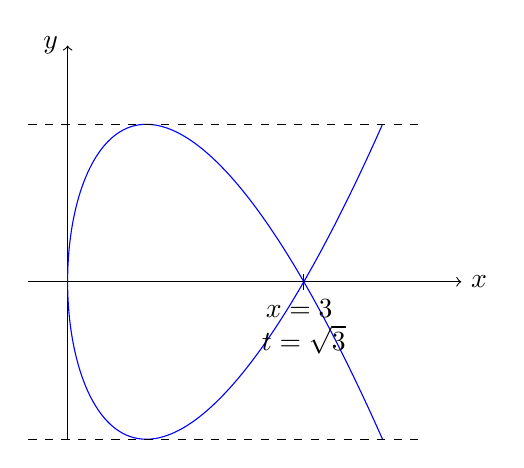
\begin{tikzpicture}
	\draw[->] (0, -2) -- (0, 3) node [left] {$y$};
	\draw[->] (-0.5, 0) -- (5, 0) node [right] {$x$};
	\draw[smooth,samples=100,domain=-2:2, blue] plot ({\x*\x},{\x*\x*\x-3*\x});
	\draw[] (3, 0.1) -- (3,-0.1) node [below, align=center] {$x=3$ ~\\ $t=\sqrt{3}$};
	\draw[dashed] (-0.5, 2) -- (4.5, 2);
	\draw[dashed] (-0.5, -2) -- (4.5, -2);
\end{tikzpicture}

\paragraph{Exemple} \[\begin{array}{rcl}
				\gamma(t) &=& (e^t, 3e^{t+\ln(2)}-1) \\
											   &=& (x(t), y(t)) \\
		y(t) &=& 3e^{t+\ln(2)} - 1 \\
			&=& 3e^t \cdot e^{\ln(2)} - 1 \\
		 &=& 6e^t - 1 = 6 6x(t) - 1\end{array}\]

\paragraph{Exemple}

\[\gamma(t) = (3t - 6t^2 + 4t^3, 3t(1-t)), t \in \mathbb{R}\]

Point singuliers ?

\[\begin{array}{rcl}
		\gamma'(t_0) &=& 0 \\
									&=& (3-12t + 12t^2, 3 - 6t) \\
						   &=& 3((1-2t)^2, 1-2t)\end{array}\]

		pour $t= \frac{1}{2}$, $\gamma'(\frac{1}{2}) = 0, \gamma(\frac{1}{2})$ est un point singulier.

Pour obtenir la pente de la tangente en $\gamma(\frac{1}{2})$, on doit dérivé de nouveau :

\[y''(t) = 3(-4(1-2t), -2) \neq (0, 0)\]

En $\frac{1}{2}, y''(\frac{1}{2}) = (0, -6)$ : Une tangente vertical.

\begin{tikzpicture}
	\draw[->] (0, -3) -- (0, 5) node [left] {$y$};
	\draw[->] (-1, 0) -- (9, 0) node [right] {$x$};
	\draw[smooth,samples=100,domain=-2:2,blue] plot ({3*\x -6*\x*\x + 4 *\x*\x*\x},{3*\x*(1-\x)});
\end{tikzpicture}
